\documentclass[tikz,border=2pt]{standalone}

% --- 定义颜色 ---
\definecolor{midOrange}{HTML}{F57C00}

\begin{document}
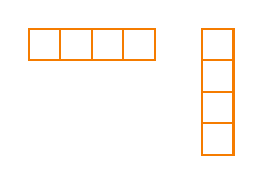
\begin{tikzpicture}[
    % 定义统一的线条样式
    border_style/.style={thick}
]

    % --- 绘制宏 ---
    \newcommand{\yd}[4]{
        \node[inner sep=0] (#1) at (#2) {};
        \begin{scope}[shift={(#1.north west)}]
            \foreach \row [count=\r] in {#3} {
                \foreach \col in {1,...,\row} {
                    % 使用指定的颜色绘制边框,不填充
                    \draw[color=#4, border_style] (0.4*\col-0.4, -0.4*\r+0.4) rectangle ++(0.4, -0.4);
                }
            }
        \end{scope}
    }

    % --- 绘制图形 (紧凑排列) ---

    % 1. Partition [4] (横条) 放在原点
    \yd{p4}{0,0}{4}{midOrange}

    % 2. Partition [1,1,1,1] (竖条) 放在右侧紧凑位置
    % [4]的宽度是 4*0.4 = 1.6cm。我们在 2.2cm 处放置下一个,间距为 0.6cm
    \yd{p1111}{2.2,0}{1,1,1,1}{midOrange}

\end{tikzpicture}
\end{document}